\documentclass[dissertation.tex]{subfiles}
\begin{document}

Neural Networks (NN) are an extremely successful tool, they are widely adopted
commercially and closely studied academically, however even given the attention
they have there is no comprehensive understanding of how these models generalize
data and provide such impressive performance -- in fact very little is known
about how NN learn or about their inner workings. Recently Prof.\ Tishby
\cite{TISHBY} produced a paper claiming to understand the basic principles of
how NN work. He decided to examine NNs through the information domain. Tishby
made the claim that the incredible performance of NNs is due to their ability to
compress information. Compressing data means the network is only able to keep
relevant input features and it must discard the irrelevant bits of information,
leading to ability to generalize. 

Tishby made interesting claims and provided experimental evidence to support his
claims, however he did not provide a formal proof leaving his results up for
debate. A paper release by Saxe \cite{SAXE} has contested the claim made by
Tishby arguing that compression cannot happen in Neural Networks and the results
are a consequence of the hyper parameters Tishby used. However, Saxe's paper
suffers from the same problem as Tishby's as it does not provide a formal proof
only experimental evidence -- as such ti does not settle the rebuttal.  To fully
understand the discussion we need to understand the following topics Entropy and
Mutual Information, Neural Networks, and Information Plane, described in
\autoref{sec:EaMI}, \autoref{sec:NN}, and \autoref{sec:IP}.

\section{Entropy and Mutual Information}
\label{sec:EaMI}

\subsection{Entropy}
\textbf{Entropy} -- quantifies information content of a random variable. It is
generally measured in bits and can be though of as the expected information
content when we sample a random variable once. Let $X$ be a discrete random
variable that can take values in $\{x_1,...,x_n\}$. $H(X)$, the entropy of
$X$, is defined by \autoref{eq:entropy}.

\begin{equation}
  H(X)=-\sum _{i=1}^{n}{P (x_i)\log P(x_i)}
\label{eq:entropy}
\end{equation}

Consider a random variable $Y$ s.t $P(Y=1) = P(Y=0) = 0.5$, \autoref{eq:entropy}
defines $H(Y)$ to be 1.

Similarly for a random variable $Y$ s.t $P(Y=0) = 0.5, P(Y=1) = P(Y=2) = 0.25$,
we have $H(Y) = 1.5$.

\subsection{Conditional Entropy}
\textbf{Conditional Entropy} -- quantifies the amount of information needed to
describe an outcome of variable $Y$ given that value of another random variable
$X$ is already known. Conditional Entropy of $Y$ given $X$ is written as
$H(Y|X)$. Let $X$ be defined as before, Let $Y$ be a discrete random variable
that can take values in $\{y_i,...,y_n\}$. The conditional entropy $H(Y|X)$ is
defined by \autoref{eq:condEntropy}.

\begin{equation}
H(Y|X)\ =-\sum _{x\in {X},y\in {Y}}P(x,y)\log {\frac {P(x,y)}{P(x)}}
\label{eq:condEntropy}
\end{equation}

Let the correlated variables $X$ and $Y$ be defined by \autoref{t:prob}.
\begin{table}[H]
  \centering
    \begin{tabular}{c|c|c}
      \diagbox{X}{Y} & 0 &1   \\
    \hline			
       0   &0.25&0.25 \\
    \hline			
       1   &0.5 &0 \\
  \end{tabular}
  \caption{Joint probability distribution for $X$ and $Y$}
  \label{t:prob}
\end{table}
\autoref{eq:entropy} and \autoref{eq:condEntropy} defines entropy values to be:
\begin{align}
  H(Y|X) &= 0.5 \nonumber \\
  H(X|Y) &\approx 0.6887 \nonumber \\
  H(X) &= 1 \nonumber \\
  H(Y) &\approx 0.8112 \label{eq:computedEntropies}
\end{align}

\subsection{Mutual Information}
\textbf{Mutual Information (MI)} -- measures how much information two random
variables have in common. It quantifies information gained about one variable
when observing the other.  \autoref{eq:miExplicit} and \autoref{eq:miEntropy}
are two examples of how we can compute MI, using explicit probability
computations or entropies of the random variables respectively, here $X$ and $Y$
are as previously defined.

\begin{equation}
      I(X,Y)=\sum _{y\in Y}\sum _{x\in X}{P(x,y)\log {\left({\frac
      {P(x,y)}{P(x)\,P(y)}}\right)}} 
\label{eq:miExplicit}
\end{equation}

\begin{equation}
  I(X, Y) = H(X) - H(X|Y)
\label{eq:miEntropy}
\end{equation}

For example of MI consider the random variables $X$ and $Y$ as
before in the conditional entropy section -- defined by \autoref{t:prob}. 

We computed the entropy values in \autoref{eq:computedEntropies}, we will use
them in \autoref{eq:miEntropy} to compute $I(X,Y)$.
\begin{equation}
  I(X,Y) = H(X) - H(X|Y) \approx 1 - 0.6887 = 0.3113
\end{equation}

\subsubsection{Properties of Mutual Information}
There are some important properties of MI that we need to take note of. Let $X$
and $Y$ be any probability distributions then:

\subparagraph{Commutative} 
\begin{equation}
  I(X,Y) = I(Y, X)
\end{equation}
\subparagraph{Information Loss} MI of two random variables cannot exceed entropy
of either of them.
\begin{align}
  H(X) \geq I(X,Y) \nonumber \\
  H(Y) \geq I(X,Y)
  \label{eq:MIloss}
\end{align}
\subparagraph{Data Processing Inequality} Let u be some function; then,
\begin{equation}
  I(X,Y) \geq I(X, u(Y))
\end{equation}
\subparagraph{Invertible Transformation} Let u be some invertible function;
then,
\begin{equation}
  I(X, Y) = I(X, u(Y))
\end{equation}

\section{Neural Networks}
\label{sec:NN}

Before we understand neural networks we need to understand The Prediction
Problem and the purpose of Machine Learning Frameworks.

\subsection{The Prediction problem} 

Suppose we have some dataset $D$ defined as $(x_i, y_i)$ for $i = 1,...,N$. The
prediction problem is finding a function $f$ s.t \autoref{eq:prediction} is
satisfied.
\begin{equation}
  f(x_i) = y_i \text{ for } i = 1,...,N
  \label{eq:prediction}
\end{equation}
Prediction task is a common task that involves having input data
$\{x_i,...,x_N\}$ and finding the label, some desirable feature,
$\{y_i,...,y_N\}$. 

The prediction problem could be simple to extract: for example if our input is a
natural number $x_i\in\mathbb{N}$, and our label is either $true$ or $false$
depending if $x$ is even or odd -- in which case function defined by
\autoref{eq:evenodd} satisfies the problem.  \begin{equation}
  g(x) = \begin{cases}
    True, & \text{if } \exists n\in\mathbb{N}.x = 2n , \\
    False, & \text{otherwise}.
  \end{cases}
\label{eq:evenodd}
\end{equation}
The prediction problem also can be impossible to solve: for example the halting
problem, if our $x's$ are programs and $y's$ boolean values corresponding if the
program halts or not.


Of course the prediction problem can be hard or impossible to solve as is the
case for problems:
\begin{table}[H]
  \centering
    \begin{tabular}{l|l|l}
      input data & label & difficulty \\ 
      \hline
      \rowcolor{Gray}
      medical symptoms & diagnosis & intractable \\ 
      picture  & object in the picture &  \\ 
      \rowcolor{Gray}
      face photograph  & identity &  \\ 
      stock market history  & future stock prices &  \\ 
      \rowcolor{Gray}
      program  & does the program halt & proved to be unsolvable \\ 
      boolean equation  & is the equation satisfiable & expensive to compute 
  \end{tabular}
  \caption{Example of specific prediction problems }
  \label{t:prediction}
\end{table}

Problems listed in \autoref{t:prediction} are either intractable, unsolvable or
too expensive to compute -- hence we cannot produce an algorithm that always
give the correct answer and runs in a reasonable time.

\subsection{Machine Learning Frameworks}

If the Prediction problem is too difficult and we are tolerant to errors in our
labels we may want to use a supervised machine learning framework\footnote{In
this thesis we are exclusively talking about supervised machine learning
techniques -- the word "supervised" will be omitted for brevity} to tackle the
problem. 

Every machine learning framework requires that we have some subset
$\hat{X}\subseteq\{x_i,...,x_N\}$ s.t that $ \forall x\in\hat{X}$ we know label
the $y$. A framework uses the data in order to reach some goal -- such as
minimizing the prediction error. The way any machine learning framework learns
from data varies, but generally more data means an increase in prediction
performance.

\subsection{Neural Networks} 

\textbf{Neural Networks (NN)} are an example of a machine learning framework. They learn
from data and attempt to solve the prediction problem.

The structure of a NN consists of layers of nodes, where every consecutive
layer is fully connected as in \autoref{fig:nnOriginal}.  When we try to
predict a label of a specific input every node gets assigned a value in the
real number space $\mathbb{R}$. Values for the Input nodes are provided,
whereas values for the nodes in non-input layers are generated based on nodes
from the preceding layer. Let $n_{l,i}$ be the value that the $i'th$ node in
layer $l$ takes. Let $w_{l,j,i}$ be a parameter that influences how relevant
the $j'th$ node in layer $l$ is to the $i'th$ node in layer $l+1$.
\begin{equation}
  n_{l+1,i} = g(\sum_{j = 0}^{\text{layer }l\text{ size}} w_{l,j,i}*n_{l,j})
  \label{eq:nextNode}
\end{equation}
$g$ in \autoref{eq:nextNode} is called the activation function and is generally 
taken to be:
\begin{itemize}
  \item{
      Leaky ReLu: 
      \begin{equation*}
        g(x) = \begin{cases}
          x, & if x > 0 \\
          \alpha{x}, & \text{otherwise}.
        \end{cases}
      \end{equation*}
      $\alpha$ here is some small value such as $\alpha = 0.01$
    }
  \item{
      Sigmoid: $g(x) = \frac{1}{1+e^x}$
    }
  \item{
      Tanh: $g(x) = tanh(x)$
    }
\end{itemize}


\subparagraph{Stochastic Gradient Descent (SGD)} The NNs training algorithm is
called Stochastic Gradient Descent. SGD periodically adjusts the parameters $w$
according to some goal such as minimising the prediction error. 

SGD is an iterative process -- it introduces a notion of epochs where one
iteration of the algorithm advances the epochs by one. Notion of epochs implies
that the parameters $w$ depends on which epoch we are currently at -- thus it
must take the epoch number $e$ as an argument -- $w(e)$.


\begin{figure}[H]
  \centering
  \begin{subfigure}[t]{0.49\textwidth}
    \centering
    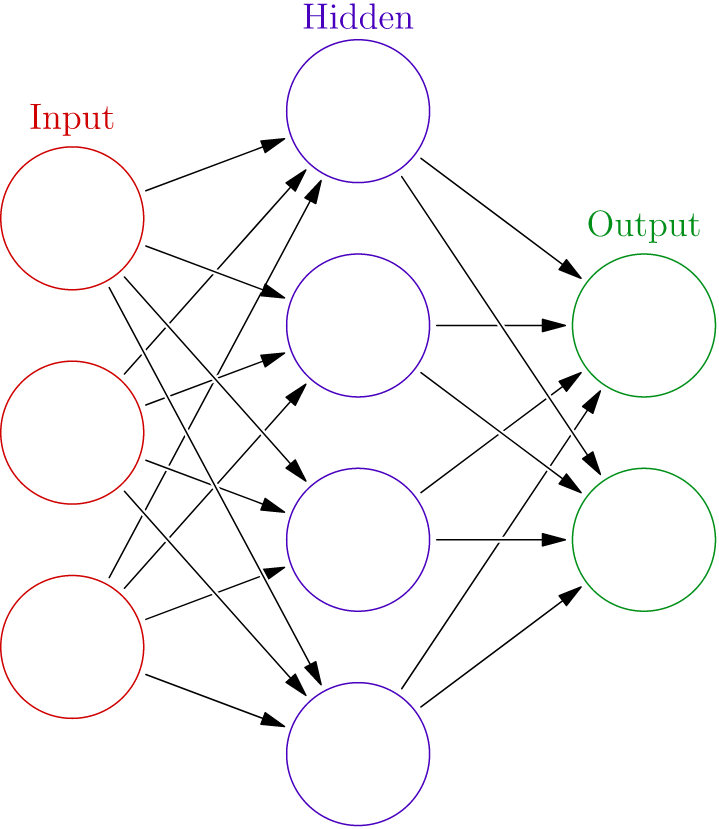
\includegraphics[width=0.7\textwidth]{figs/neural_network.png}
    \caption{
      Structure of a typical neural network.
    }
    \label{fig:nnOriginal}
  \end{subfigure}
  \hfill
  \begin{subfigure}[t]{0.49\textwidth}
    \centering
    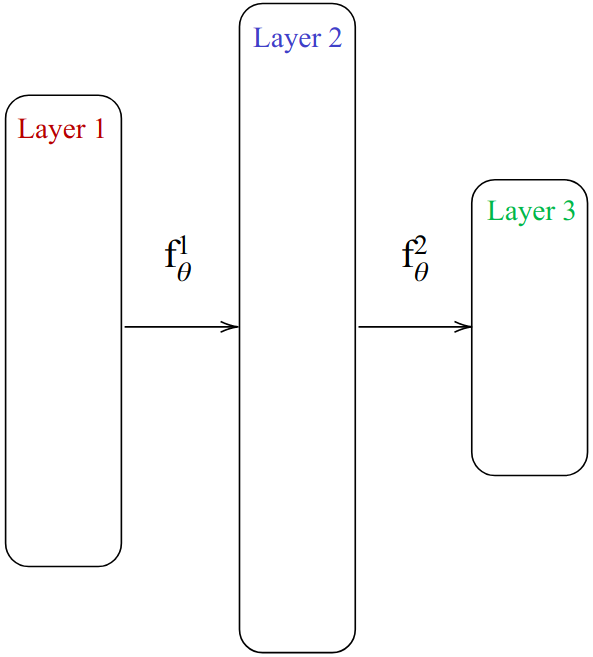
\includegraphics[width=0.7\textwidth]{figs/neural_network_abstraction.png}
    \caption{
      Structure of our abstracted neural network.
    }
    \label{fig:nnModified}
  \end{subfigure}
    \caption{
      Source: Wikimedia Commons 
    }
\end{figure}

\subsection{Abstracting the Neural Network}
For our purposes we will abstract away the individual nodes in the NN and only
consider the layer structure -- as in \autoref{fig:nnModified}.

In our abstraction the NN is structured in layers where every layer holds
an intermediate representation of the final prediction output - let us call this
intermediate representation an \textbf{activation} of that specific layer.
We will formally define a neural network with $L$ layers to be a sequence of $L$
functions $f_{\theta(e)}^1,f_{\theta(e)}^2,...,f_{\theta(e)}^L$ that are
parameterized by $\theta$ s.t. Equations \ref{eq:nnTransitions} hold.
In our abstract the parameters $\theta$ correspond to the parameters $w$,
therefore $\theta$ depends on the current epoch -- $\theta(e)$.
Let us also define an \textbf{activation} of layer $l$ to be output of the
function $f_\theta^l$.

\vbox{
\begin{align}
	\text{let } t_0 &= x, \nonumber \\
  t_0 \rightarrow f_{\theta}^1(t_0) &= t_1, \nonumber \\
  t_1 \rightarrow f_{\theta}^2(t_1) &= t_2, \nonumber \\
  &... \nonumber \\
  t_{L-1} \rightarrow f_{\theta}^L(t_{L-1}) &= t_L, \nonumber\\
  \text{let } \hat{y} &= t_L \label{eq:nnTransitions}
\end{align}
\vspace*{-\baselineskip}
\vspace*{-\baselineskip}
\begin{gather}
  \text{values } t_1,t_2,...,t_L 
  \text{ here are } \textbf{activations } \text{of layers } 1,2,...,L,
	\nonumber\\
	x \text{ is any input to the NN from the set } \{x_i,...,x_N\}, \nonumber\\
	\hat{y} \text{ is the prediction of the NN for the input,} x
	\text{ which may or not be correct label,} \nonumber\\
	\text{the arrow `}\rightarrow\text{' signifies a transition from one NN layer to another.}
	\nonumber
\end{gather}
}

We now have one function for each layer transition of the NN this
allows us to extract the activation of a specific layer as in
\autoref{eq:layerL}.
\begin{gather}
  t_l = f_{\theta}^l(f_{\theta}^{l-1}(...(f_{\theta}^1(x))))
  \label{eq:layerL} \\
  \textbf{activtion}\text{ of later }l\text{ for input }x \nonumber
\end{gather}
Let us define $F_\theta^t$ to be the activation of layer $l$ given input x
i.e
\begin{equation}
  F_{\theta}^l(x) = f_{\theta}^l(f_{\theta}^{l-1}(...(f_{\theta}^1(x))))
  \label{eq:bigF}
\end{equation}

\autoref{fig:network} summarizes our NN definition.

\vbox{
\begin{center}
\end{center}



\tikzset{every picture/.style={line width=0.75pt}} %set default line width to 0.75pt        

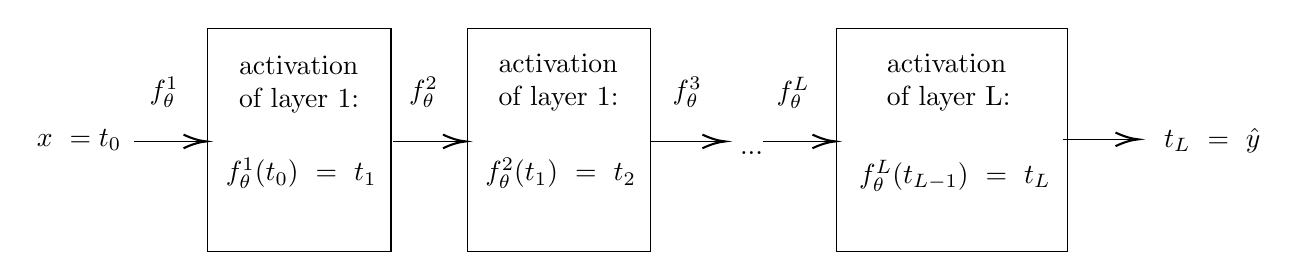
\begin{tikzpicture}[x=0.75pt,y=0.75pt,yscale=-1,xscale=1]
%uncomment if require: \path (0,244.52349853515625); %set diagram left start at 0, and has height of 244.52349853515625

%Shape: Rectangle [id:dp11557839760136379] 
\draw   (86,115) -- (174.28,115) -- (174.28,222.54) -- (86,222.54) -- cycle ;
%Straight Lines [id:da1142035093360374] 
\draw    (50.28,169.54) -- (83.28,169.54) ;
\draw [shift={(85.28,169.54)}, rotate = 180] [color={rgb, 255:red, 0; green, 0; blue, 0 }  ][line width=0.75]    (10.93,-3.29) .. controls (6.95,-1.4) and (3.31,-0.3) .. (0,0) .. controls (3.31,0.3) and (6.95,1.4) .. (10.93,3.29)   ;

%Straight Lines [id:da3402708303870947] 
\draw    (299.28,169.54) -- (333.28,169.54) ;
\draw [shift={(335.28,169.54)}, rotate = 180] [color={rgb, 255:red, 0; green, 0; blue, 0 }  ][line width=0.75]    (10.93,-3.29) .. controls (6.95,-1.4) and (3.31,-0.3) .. (0,0) .. controls (3.31,0.3) and (6.95,1.4) .. (10.93,3.29)   ;

%Straight Lines [id:da9984222042248518] 
\draw    (498.28,168.54) -- (532.28,168.54) ;
\draw [shift={(534.28,168.54)}, rotate = 180] [color={rgb, 255:red, 0; green, 0; blue, 0 }  ][line width=0.75]    (10.93,-3.29) .. controls (6.95,-1.4) and (3.31,-0.3) .. (0,0) .. controls (3.31,0.3) and (6.95,1.4) .. (10.93,3.29)   ;

%Shape: Rectangle [id:dp7529094555455995] 
\draw   (211,115) -- (299.28,115) -- (299.28,222.54) -- (211,222.54) -- cycle ;
%Straight Lines [id:da3983438928921348] 
\draw    (175.28,169.54) -- (208.28,169.54) ;
\draw [shift={(210.28,169.54)}, rotate = 180] [color={rgb, 255:red, 0; green, 0; blue, 0 }  ][line width=0.75]    (10.93,-3.29) .. controls (6.95,-1.4) and (3.31,-0.3) .. (0,0) .. controls (3.31,0.3) and (6.95,1.4) .. (10.93,3.29)   ;

%Shape: Rectangle [id:dp3082851546438703] 
\draw   (389,115) -- (500.28,115) -- (500.28,222.54) -- (389,222.54) -- cycle ;
%Straight Lines [id:da29571517496636934] 
\draw    (353.28,169.54) -- (386.28,169.54) ;
\draw [shift={(388.28,169.54)}, rotate = 180] [color={rgb, 255:red, 0; green, 0; blue, 0 }  ][line width=0.75]    (10.93,-3.29) .. controls (6.95,-1.4) and (3.31,-0.3) .. (0,0) .. controls (3.31,0.3) and (6.95,1.4) .. (10.93,3.29)   ;


% Text Node
\draw (65,146) node   {$f^{1}_{\theta }$};
% Text Node
\draw (130,142) node  [align=left] {activation \\of layer 1: };
% Text Node
\draw (131,185) node   {$f^{1}_{\theta }( t_{0}) \ =\ t_{1}$};
% Text Node
\draw (24,169) node   {$x\ =t_{0}$};
% Text Node
\draw (348,175) node   {$...$};
% Text Node
\draw (317,146) node   {$f^{3}_{\theta }$};
% Text Node
\draw (570,169) node   {$t_{L} \ =\ \hat{y}$};
% Text Node
\draw (190,146) node   {$f^{2}_{\theta }$};
% Text Node
\draw (255,141) node  [align=left] {activation \\of layer 1: };
% Text Node
\draw (256,185) node   {$f^{2}_{\theta }( t_{1}) \ =\ t_{2}$};
% Text Node
\draw (368,146) node   {$f^{L}_{\theta }$};
% Text Node
\draw (443,141) node  [align=left] {activation \\of layer L: };
% Text Node
\draw (446,186) node   {$f^{L}_{\theta }( t_{L-1}) \ =\ t_{L}$};


\end{tikzpicture}
\begin{center}



\end{center}

\vspace*{-\baselineskip}
\vspace*{-\baselineskip}
\begin{figure}[H]
  \centering
  \caption{
    Visualization of a neural networks structure. $x$ here is any input to the
    network from the set $\{x_i,...,x_N\}$.  $\hat{y}$ is the prediction of the
    network for the input $x$ which may or may not be to the correct label. The
    values $t_1,...,t_L$ here are \textbf{activations} of layers $1,...,L$.
  }
  \label{fig:network}
\end{figure}
}

\section{The Information plane}
\label{sec:IP}
The information plane is a way of visualizing the Neural Network's
training process through the information domain. Meaning we are looking
what information the NN is retaining throughout the layers, and how the
information retained changes throughout the training process.

We are interested see what information about the input and the label is retained
-- as having this information would help us understand how the neural network
learns.  Suppose we have this data available then we can examine this data with
respect to:
\begin{itemize}
  \item{
      Epochs -- lets us ask questions such as:
      \begin{itemize}
        \item{
            Is the network getting rid of noise in the network.
          }
        \item{
            Does the network ever retain all the information about the label.
          }
        \item{
            If the network does retain all the information about the label does
            training it after the point lead to performance increase.
          }
      \end{itemize}
    }
  \item{
      Layer -- lets us ask questions such as:
      \begin{itemize}
        \item{
            Is there a difference between how much information the layers are
            discarding.
          }
        \item{
            How does the information dynamics change if we add more layers.
          }
      \end{itemize}
    }
\end{itemize}

Suppose we are examining a specific NN. At the start of the training process we
expect the network to perform poorly -- meaning it does not retain information
about the label. Through the training process we expect: 
\begin{itemize}
  \item{
      The information about the label to rise until it saturates. If we train
      past this saturation point we don't expect the information about the label
      to change much.
    }
  \item{
      The information about the input to rise until we have saturated the
      information about the label. At this point we either expect:
      \begin{itemize}
        \item{
            The information about the input to keep rising if we believe the
            network starts to learn noise about the data.
          }
        \item{
            The information about the input to start reducing until the networks
            does not retain any noise about the input if we believe the network
            generalizes the data.
          }
      \end{itemize}
    }
\end{itemize}

Ideally a neural network would retain all the information relevant to the label
and none of the noise inherent in the input.

\subsection{Setup}
\label{subIPsetup}

We want to compute what information about the label and the input the network is
retaining -- that is we want to compute the mutual information:
\begin{itemize}
  \item{
      Between the input distribution and all of the network layers,
    }
  \item{
      Between the label distribution and all of the network layers.
    }
\end{itemize}

In order to compute the needed MI values we need to define the probability
distributions:
\begin{itemize}
  \item{
      $X$ - probability distribution of the input,
    }
  \item{
      $Y$ - probability distribution of the label,
    }
  \item{
      $T_{e,l}$ - probability distribution of the layer $l$ for the epoch $e$.
    }
\end{itemize}

The routine in \autoref{fig:rxty} defines the correlated random variables:
$X,T_{e,l},Y$. The probability distributions define the needed MI values:
$I(X, T_{e,l})$ and $I(Y, T_{e,l})$.

\begin{figure}[H]
    \begin{pythonfigure}
      def rxty(e, l):
        pick i ;$\sim$; Uniform {1...N}
        return ;$(x_i, F_{\theta(e)}^l(x_i), y_i)$;
    \end{pythonfigure}
    \caption{
      Definition of correlated random variables $X, T_{e,l}$ and, $Y$. The
      Probability distributions are generated from the dataset $D=\{(x_i,
      y_i)|i=1,..,N\}$. $F_{\theta(e)}^l$ is defined by \autoref{eq:bigF}
    }
    \label{fig:rxty}
\end{figure}

\subparagraph{Input Probability Distribution} The probability distribution $X$
is generated from the input dataset $D$.  Any input dataset $D$ has an inherent
probability distribution but most of the time we don't know it exactly.
\autoref{fig:rxty} makes the assumption that $D$ is uniformly distributed and
thus takes every input value to be equally likely.  If we had a specific dataset
we could adjust our assumption and assign a different probability distribution
to the input dataset.

\subsection{Visualization}

The Information Plane visualizes how the information retained in the NN changes
throughout the training period. 
In order to do this we need values $I(X,T_{e,l})$ and $I(Y,T_{e,l})$, for every
epoch $e$ and every layer $l$ -- we show how we obtain them in
\autoref{subIPsetup}.

To better understand how the Information Plane present the data let us consider
\textbf{\autoref{fig:Ip1}} -- it shows the Information Plane for a NN for the
first epoch before any training has been done. This implies that parameters
$\theta(e)$ have not been affected by SGD and are thus random. If the network is
random we would expect it not be able to retain much information.  In the image
we see that the network loses almost all information about the label $I(Y,
T_{1,5}) \approx 0$, but retains some information about the input $I(X, T_{1,5})
\approx 3$ -- we can see that this random NN only retains noise.

Let us now bring our attention to \textbf{\autoref{fig:Ip2}} -- it shows a NN
that was trained for $\approx{10^4}$. The NN was initialized with random
parameters $\theta(1)$, then trained via the SGD algorithm which altered the
parameters $\theta$. The NN was trained so we expect to see a rise of mutual
information with the label $I(Y, T_{e, l})$, throughout the training period --
and we do see this in the Figure. However, we also see some other interesting
features:
\begin{itemize}
  \item{
      Notice that the increase in $I(Y,T_{e,l})$ is very rapid at the start of
      the training period, but slows down considerably after $\approx 1000$
      epochs. The rapid increase might be the NN learning features that are
      highly correlated with the label, hence easy to learn.
    }
  \item{
      Notice how when increase in $I(Y,T_{e,l})$ slows down we start to see a
      decrease in the information about the input -- $I(X,T_{e,l})$. This might
      be the point when the networks starts to remove the noise from the input.
    }
  \item{
      Notice how in both figures the NNs retain all the information about the
      label -- This suggest that in order to achieve high performance retaining
      all the information is not enough. If all we needed to do is retain all
      the label information there would be no reason to add more layers to the
      neural network.
    }
\end{itemize}

\begin{figure}[H]
  \centering
  \begin{subfigure}[t]{0.48\textwidth}
    \centering
    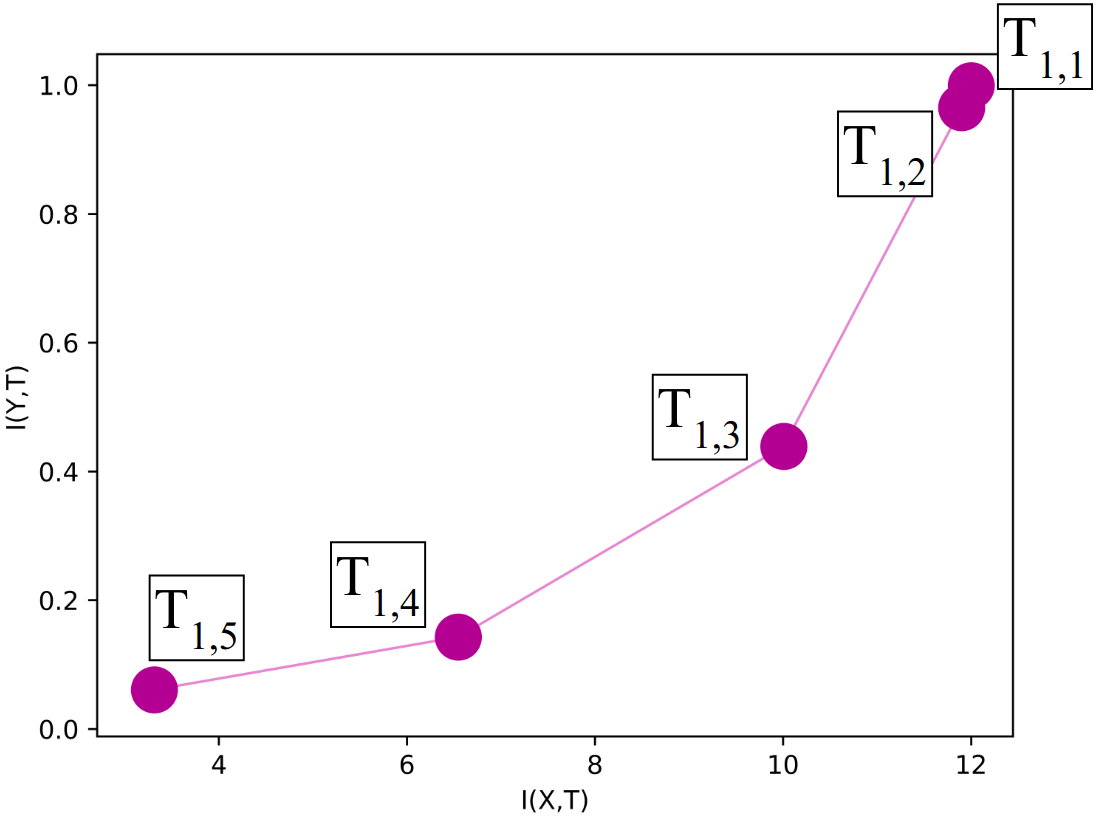
\includegraphics[width=\textwidth]{figs/ip_1v3.png}
    \caption{
      information plane for a neural network with 5 layers, which was only trained
      for one epoch.
    }
    \label{fig:Ip1}
  \end{subfigure}
  \hfill
  \begin{subfigure}[t]{0.5\textwidth}
    \centering
    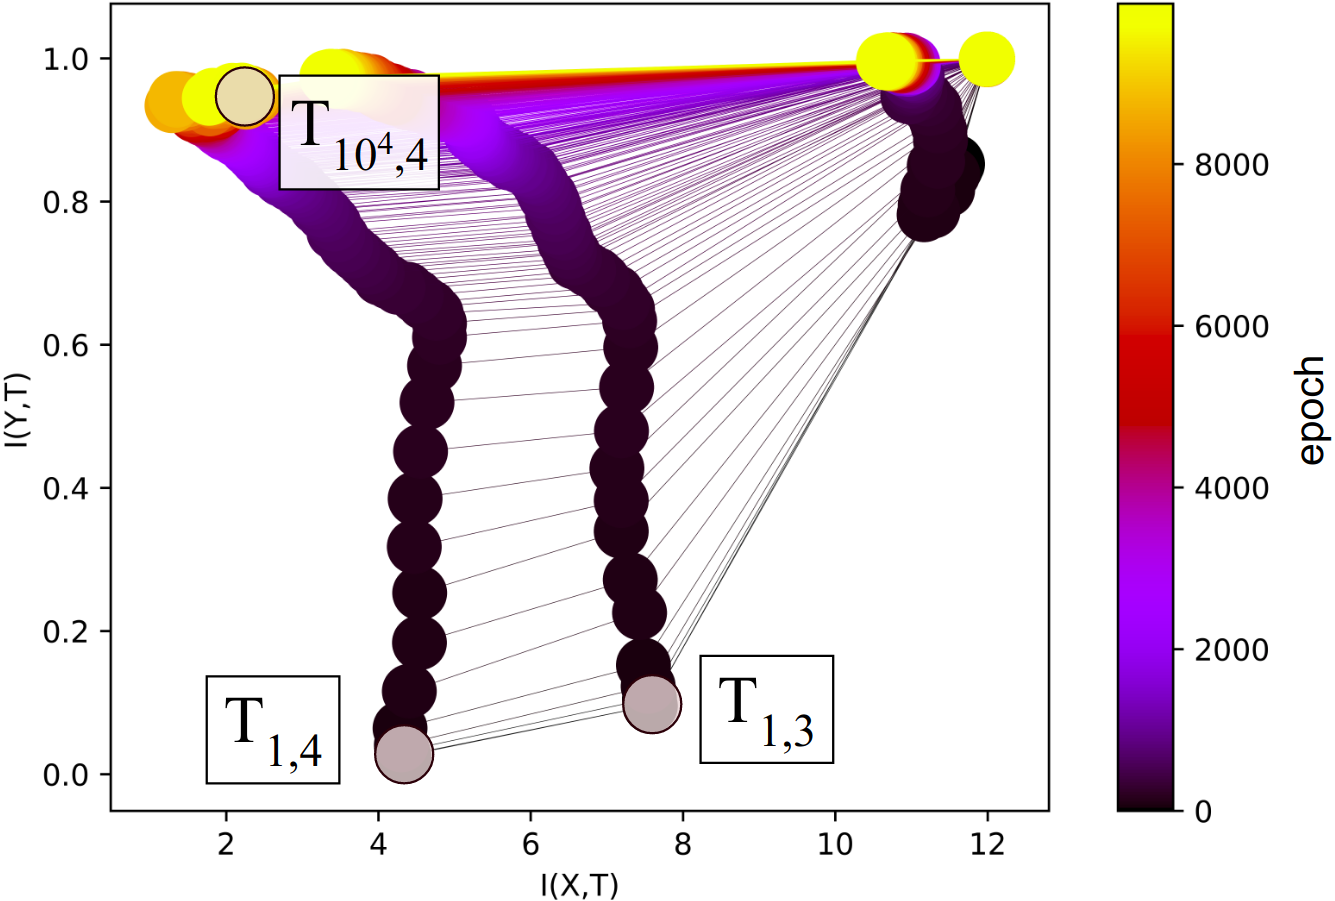
\includegraphics[width=\textwidth]{figs/ip_10000v3.png}
    \caption{
      Information plane for a neural network with 4 layers, which was trained
      for approximately $10\,000$ epochs.
    }
    \label{fig:Ip2}
  \end{subfigure}
  \caption[explaining IP]{
    The nodes in the figures correspond to information content of layers in the
    NN. The lines between the nodes help us distinguish individual epochs if
    more than one is plotted on the screen and lets us see the order of layers
    within a single epoch.
    
    Notice that some nodes are labeled $T_{e,l}$, where $e$ is the epoch number
    and $l$ is the layer the node belongs to. Consider $T_{1,3}$ from
    \autoref{fig:Ip2} -- the node corresponds to the information content of
    layer 3 for the 1'st epoch, the $x$ coordinate of the node is the value
    $I(X, T_{1,3})\approx{8}$, the $y$ coordinate is the value $I(Y,
    T_{1,3})\approx{0.1}$
   
    The Neural Networks in both figures have been trained on the same dataset as
    used by Tishby\cite{TISHBY}, The datasets input entropy, $H(X)$, is 12 and
    label entropy, $H(Y)$, is 1. Notice the $x$ and $y$ axis don't exceed the
    entropies $H(X)$ and $H(Y)$ respectively -- this is due to the information
    loss property of MI \autoref{eq:MIloss}.
  }
\end{figure}

\subsection{Interpretation of the Information Plane}

Let us once again consider \autoref{fig:Ip2} -- we can see two general phases in
the neural network. Tishby has named them \emph{The Fitting Phase} and \emph{The
Compression Phase}. 

These phases are observations made by Tishby and seem to be reproducible in by
experiments. Even though Tishby gave no clear definition of how to identify the
phases, they seem to follow the properties outlined bellow.

\subparagraph{The Fitting Phase} In \autoref{fig:Ip2} the neural network is in
the fitting phase from the start of the training up until epoch $\sim$1500. The
duration of the fitting phase varies heavily on the training parameters and is
most influenced by the size of our input dataset. The fitting phase is
characterized by:
\begin{itemize}
  \item{
      A rapid increase in $I(Y, T_{e,l})$, the information about the label, as
      we advance through the epochs $e$. The increase is especially visible in
      the later layers, in our case layers 3 and 4.
    }
  \item{
      Either an increase or no change in $I(X, T_{e,l})$, the information about
      the input, as we advance through the epochs $e$, in our case we see very
      little change in $I(X,T_{e,l})$.
    }
\end{itemize}

Tishby's understanding of the Fitting phase is that the network tries to
memorize the data and makes predictions based on the observations, this means
that the network may learn features that only superficially correlate with the
correct label.

\subparagraph{The Compression Phase} In \autoref{fig:Ip2} the neural network
enters the compression phase when the fitting phase ends around epoch $\sim$1500
and lasts until we finish the training process. The compression phase is
characterized by:
\begin{itemize}
  \item{
      A slowdown of how fast $I(Y, T_{e,l})$ is increasing with respect to epoch
      $e$. 
    }
  \item{
      A slow decrease of $I(X, T_{e,l})$ with respect to epoch $e$.
    }
\end{itemize}

Tishby's understanding of the Compression phase is that the network learns how
to compress the representation of the input. This means the network has to
discard features that do not help with predicting the correct labels. Discarding
irrelevant features helps the neural network to generalize and produce better
prediction for new data.

\section{Testability}

Software related to NN tends to be very compact as it heavily relies on external
libraries that are extensively tested. In our case the most effective way to
test the software is to provide tools that help examine the data. I have
provided such tools in form of data visualization -- such as a tool to generate
a video of the training process, which lets a human detect anomalies.

\section{Software Engineering}

The project was build using the Spiral model. I needed to build a working
version as fast as possible in order to verify the validity of Tishby's
experiments. Once the Minimal Viable Product was build I added features as
needed. Features such as different experiments, performance optimizations,
visualization tools.

\section{Starting Point}

In order to understand the theory required I had learn the ideas presented in
papers by Tishby\cite{TISHBY}\cite{TISHBY2} and Saxe\cite{SAXE}. I had to have a
strong understanding of Neural Networks and Information Theory.

The starting for implementation was knowledge of \emph{Python 3}. For this
project I had to learn the Machine Learning Frameworks: \emph{Keras} and
\emph{Tensorflow}.

\end{document}
